\documentclass{article}

\usepackage{amssymb}
\usepackage{amsfonts}
\usepackage{amsmath}
\usepackage{dsfont}
\usepackage[a4paper, total={6in,8in}]{geometry}
\usepackage{graphicx}
\usepackage{float}
\usepackage{hyperref}

\graphicspath{{figures/}}

\title{MATH30000 Project - Phonation}
\author{Will Woolfenden}

\begin{document}

\maketitle

\section{Introduction}

\subsection{Definitions}

Phonation is the human process in which respiratory exhalation and vocal cord oscillations work together to produce sounds that we identify as spoken words.
Air is projected from the lungs in a fluid motion through the airways.
When passing through the larynx, the forced oscillations of the contained vocal cords interact with the air particles and induce the sound of speech.

The goal of this project is to explore models of the phonation process.



\section{Principles of the single-mass model}

\subsection{Derivation}

% TODO: Add figure of the model schematic

The first model we will study is taken from Theory and Measurement of Snores \cite{gavriely_jensen_1993}.
It models the inspiratory process, designed to investigate snoring as a symptom of obstructive sleep apnea.
The model proposes that the inspiratory path consists of first a region of the upper airway,
which has a given viscous resistance.
Then, there is a region of a channel between two walls of given area, where one wall is a suspended plate rather than being fixed in place.
The term we wish to investigate is $b$, which describes the positive displacement between the fixed wall and the suspended wall opposite.
The walls themselves are assumed to be of equal dimensions, and behave such that the surfaces are always parallel to each other.
Also necessary to note is that the plate may only move in the direction of $b$ which is the normal to its surface,
hence $b$ measures the only degree of freedom of the plate's motion.

%figure on diagram of the model

The oscillations in $b$ that may take place, depending on conditions, is the subject of our analysis.
In the original paper, the oscillations are regarded as snores,
whereas here they will be regarded as the production of phones.
The idea is the same, since the mathematical principles applied in the definition of the model are not exclusive in any way to particular studies of sleep apnea or the like.

Oscillations are the event where, given certain constraints, $b$ will exhibit simple harmonic motion. %maybe cite here
In the model provided, indefinite oscillations can very much be observed given the right conditions,
however it is important to be aware of some properties of the model,
namely the region in which our attention is focussed. Given physical attributes are associated with the model,
and so, for example, behaviours of $b$ when negative are ignored in the investigation.

There are three forces acting on the plate in the airway, which govern the motion we are investigating.
The plate is suspended in place by an elastic force $F_k$, namely a conventional Hooke spring with spring constant $k$.
This spring force suspends the plate such that it resists the closure of the airway,
so the tension force on the plate is acting tangent to the direction of positive displacement of the plate.

% schematic with opposing walls and illustration of spring direction.

Since the upper airway has a resistance $R$ to the inspiratory fluid flow,
this leads to a pressure drop in the airways. %TODO: Explain this

An internal increase in pressure would produce an outward force on the airway,
which in this model would be tangent to the positive displacement direction.
Since there is instead a \textit{decrease} in pressure, an inward force is resultant,
in the direction tangent to the negative displacement. We label this force as $F_p$.
Pressure itself is the force per unit area,
so the value of the force $F_p$ is the pressure multiplied by the surface area of the plate.

The final force to consider in the motion of the plate is consequence of Bernoulli's principle,
namely that along a streamline, in a steady flow\footnote{It is important to note that in the general case, the flow may not necessarily be steady.},
the sum of the kinetic energy and the potential energies are constant.
In Bernoulli's equation (Equation \ref{eqn:bernoulli}), $1/2\mathbf{u}\cdot\mathbf{u}$ is the fluid kinetic energy,
$\Omega$ is the potential energy per unit mass of the body forces of the fluid,
and $\int dp/\rho$ is the inner potential energy, regarding that $p$ and $\rho$ are either constant or codependent.
$\Omega$ is often referred to as the material derivative.

\begin{equation}
    \frac{1}{2}\mathbf{u}\cdot\mathbf{u} + \Omega + \int\frac{dp}{\rho} = C
    \label{eqn:bernoulli}
\end{equation}

%this is where the explanation gets dodgy - this could be completely wrong. if so, then the bernoulli effect force is more likely the increase in fluid ke when a constriction leads to an increase in pressure
In order to obtain the pressure consequent of Bernoulli's principle, we simply rearrange the equation for $p$.
We obtain $F_b$ by again multiplying the pressure by the cross-sectional area of the plate.

%include some derivation for $P_b$?

The governing equation of the model is derived from Newton's second law.
Given that the plate has a mass $m$, we know the three forces acting on it,
and so the initial equation of motion can be expressed as

\begin{equation}
    m\frac{d^2 x}{dt^2} = F_e - F_p - F_b.
    \label{eqn:model_init}
\end{equation}

This is not the principal equation of the model,
since the terms should be nondimensionalised and normalised.
For example, $x$ measures displacement,
but it is not stated under what scale.
Furthermore, the terms for the forces are all products of pressure and their dimensional properties,
meaning they measure in units that would ideally be reduced.
We can normalise $x$ by defining $b = x/x_0$, where $x_0$ is the resting position of the plate under particular circumstances. %TODO: amend this!! what are the particular circumstances??
The forces can be nondimensionalised by dividing by the areas or volumes they are acting over.
Resultingly, we produce the governing equation for the positive displacement of the channel wall from collapse at $0$,

\begin{equation}
    \frac{d^2b}{dt^2} = 1 - q - b - \frac{\mu q^2}{2b^2}
    \label{eqn:master}
\end{equation}

where $\mu, q$ are parameters linked to the forces acting on the channel wall.

%plan is to have this chapter just discuss individual properties of the model with analysis where relevant. Will include matrix method. Then in next chapter we introduce KE graphs in the phase-plane.

\subsection{Nonlinearity}

It is important to note the properties of Equation \ref{eqn:master} before developing analysis.
The equation itself is a second order, nonlinear, autonomous, inhomogeneous ODE.
The property of nonlinearity is due to the existence of the $\mu q^2/2b^2$ term.
Due to the equation being nonlinear, regular methods for solving ODEs are far less powerful,
and the properties of solutions are different to regular linear ODEs.
Most importantly, while linear ordinary differential equations often possess unique solutions subject to boundary or initial conditions,
the same does not apply in the case of nonlinear equations.

We will first demonstrate the implications of nonlinearity by attempting methods suitable for linear ODEs,
in which we do not expect to solve the ODE but instead use for demonstration.
Note the absence of the $db/dt$ term in the governing equation.
We can attempt the method of reduction by proposing a substitution $v=db/dt$ and forming a first order ODE.
First, note that

\begin{equation}
    \frac{dv}{dt} = \frac{dv(b(t))}{dt} = \frac{dv}{db}\frac{db}{dt} = \frac{dv}{db}v,
\end{equation}

and hence (with an abusive assumption of commutativity),

\begin{equation}
    v \frac{dv}{db} = 1 - q - b - \frac{1}{2}\mu q^2\left( \frac{1}{b^2} \right).
\end{equation}

Assuming we can separate the variables, we can write an indefinite integral equation and obtain an expression for $v$, namely

\begin{equation}
    \begin{aligned}
        \int v~dv                                      & = \int \left(1 - q - b - \frac{1}{2}\mu q^2\left( \frac{1}{b^2} \right)\right) db \\
        \Rightarrow v^2 = \left(\frac{db}{dt}\right)^2 & = 2b(1-q) - b^2 + \mu q^2\left(\frac{1}{b}\right) + C_1,
    \end{aligned}
    \label{eqn:first_order_reduction}
\end{equation}

obtaining a constant of integration $C_1$.
We now have a first order differential equation on $b$, %however we can't solve it because no
but this equation is even harder to reduce or even solve, as we only have the form $v^2 = g(b)$,
not giving the form of the first derivative directly.
Therefore, statements of existence and uniqueness for solutions of ODEs,
which we are accustomed to,
do not hold in the situation where the differential equation is non-linear.

We could have deduced this from the explicit form of Equation \ref{eqn:master},
but this section serves for illustration to aid the reader's understanding of why we cannot analytically solve this ODE.
Additionally, the equation of the form $v^2 = g(b)$ will be useful later.

\subsection{Autonomy}

\begin{figure}
    \centering
    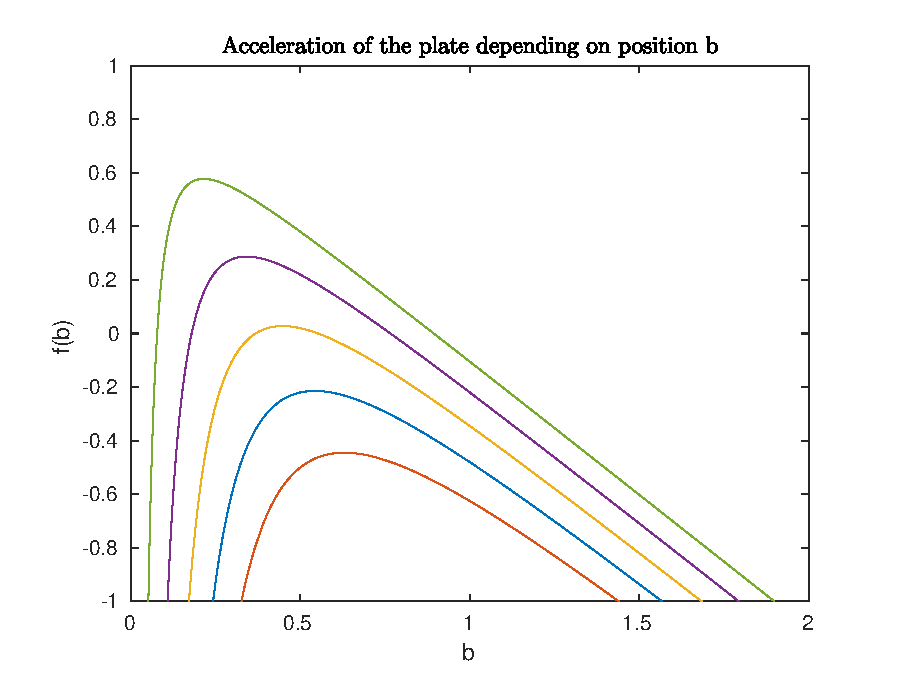
\includegraphics[width=0.5\linewidth]{f_plot_mu_1_q_vary}
    \caption{A plot of the function $f(b) = 1-q-b-\mu q^2/2b^2$ where $\mu=1$, $q$ ranging from $0.1$ to $0.5$}
    \label{fig:acc_b_plot}
\end{figure}

The reader may notice that the Equation \ref{eqn:master} is an autonomous ODE,
namely that the independent variable $t$ itself does not appear.
If we let $f$ be a function of $b$ equal to the right-hand side of the equation,
we can produce a plot of the behaviour of $f(b)$ against $b$,
and since the equation is autonomous, this behaviour is not affected by position in time.
Figure \ref{fig:acc_b_plot} shows a plot of $f(b)= 1 - q - b - \mu q^2/2b^2$ against $b$.

This plot allows us to deduce some intuition about the behaviour of $b$.
At a point $b=b_0$, the function $f(b_0)$ is equal to the outward acceleration of the plate.
We can see that $f$ tends towards negative infinity both as $b\rightarrow 0$ and as $b\rightarrow\infty$,
and that for certain $\mu, q,$ there is a positive region of $f$.
Hence if $b$ is either small or large, it will accelerate to closure,
whereas for a range of intermediate values it may accelerate outwards instead.
It is possible under certain conditions for $b$ to behave similarly to a harmonic oscillator,
where its position and acceleration move back and forth reciprocally.

Note that the plot of $f(b)$ does not account for velocity.
Different initial conditions could cause $b$ to behave differently under the same acceleration.

We will start by analysing the properties of the $f(b)$ curve.
In order for there to exist a region of $f(b)$ that takes positive values,
the local maximum of $f(b)$ must be greater than zero.

\begin{align}
    f(b)              & = 1 - q - b - \frac{\mu q^2}{2b^2} \\
    \Rightarrow f'(b) & = -1 + \frac{\mu q^2}{b^3},
\end{align}

from which we can deduce that the maximum is located at the point where $b^3 = \mu q^2$.
If we plug this back into $f$, we can deduce the condition

\begin{align}
    f((\mu q^2)^{\frac{1}{3}}) & = 1 - q - (\mu q^2)^{\frac{1}{3}} - \frac{\mu q^2}{2(\mu q^2)^{\frac{2}{3}}} \\
                               & = 1 - q - \frac{3}{2}(\mu q^2)^{\frac{1}{3}}.
\end{align}

We obtain the result

\begin{equation}
    1 - q - \frac{3}{2}(\mu q^2)^{\frac{1}{3}} > 0.
    \label{eqn:osc_condition}
\end{equation}

If Equation \ref{eqn:osc_condition} is satisfied,
then there exists a region of $f$ which is positive.
Hence if this condition is met then oscillations may occur. %% I feel this should be more rigorous - we haven't proved that this is the condition for oscillations to occur.
We have not yet provided the results to justify this statement, but in the next section we will provide rigorous arguments. % this is my backup argument for now.
Further on, we will be regularly making the assumption that this condition is satisfied,
and hence that oscillations can occur,
in order to develop our analysis of the model.

% Clearly $f$ represents acceleration of the movable wall as a function of displacement $b$. We are only ever concerned with positive $b$ due to the assumptions of the model.
% $f'$ is monotone decreasing, so there may be an interval $I_0=(p,q)$ such that if $b\in I_0$
% then $f$ is positive i.e. $p,q$ are the zeroes of $f$.
% It is not certain that $f$ will have a positive region,
% and this is decided by the parameters $\mu$ and $q$.
% Particularly, we require that the maximum of $f$ ($f'(b_c) = 0$) is greater than zero:

If the acceleration of the channel wall is positive, then the wall will accelerate outwards,
however the acceleration will have to oscillate from positive to negative in order for there to be oscillations in the position itself.
Unlike the simple harmonic oscillator $d^2 x/dt^2 + x = 0,$ the values of $b$ we consider are strictly positive.

\section{Computation of the single-mass model}

%introduce the parameter space
%first discuss configuring the system of differential equations in MATLAB
%introduce phase portrait to compare with distance/time
%integral to the kinetic energy curve graph, recalling earlier result
%matrix method with eigenvectors in the phase plane

%after this is the chapter on developing the single mass model.
%damping
%we assumed steady bernoulli flow for an unsteady problem

\subsection{The parameter space}

\begin{figure}
	\centering
	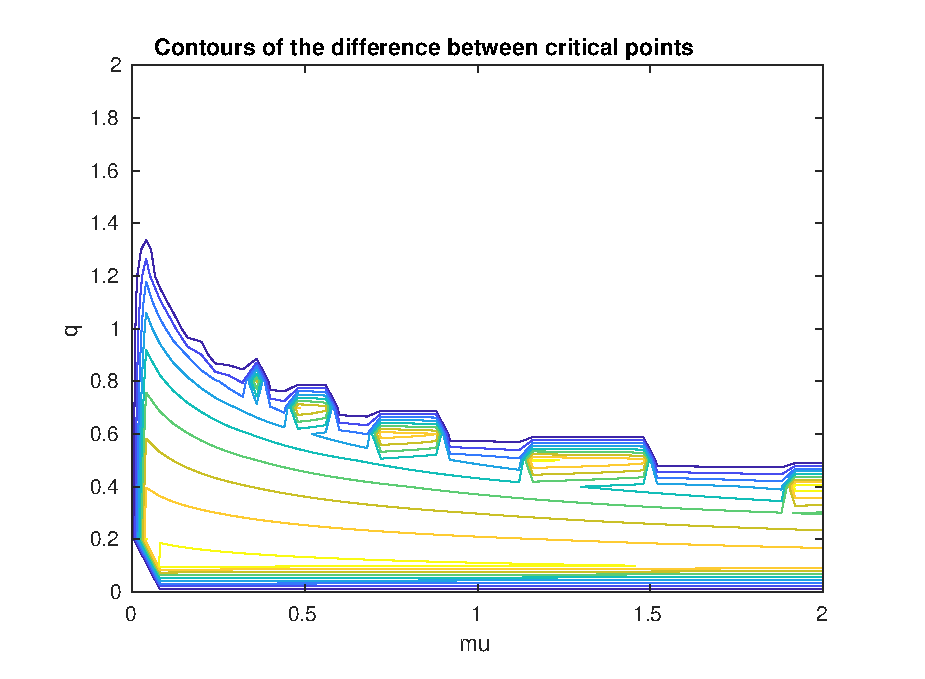
\includegraphics[width=0.5\linewidth]{param_space}
	\caption{A contour graphic of the parameter space. The displacement of $Z$ over a point $(\mu,q)$ represents the distance between critical points for the corresponding form of Equation \ref{eqn:master}.}
	\label{fig:param_space}
\end{figure}

Recall the result obtained in Equation \ref{eqn:osc_condition}.
We can produce a graph (see Figure \ref{fig:param_space}) where $\{\mu, q\}$ is the basis for the plane, and plot the distance between points.
Note that, by the properties of the derivation of the model,
$\mu$ and $q$ must be strictly positive,
hence we are only considering points in the quarter-plane.
Any suitable form of Equation \ref{eqn:master} can be placed in this region,
and if that version exists within a particular contour,
then oscillations may occur in a region of proportional scale.
Around the edges of the curve, the points bifurcate,
which is equivalent to the curve $f(b)$ only having one real-valued zero.

We can gain interesting and useful results regarding sufficient values of $\mu, q$,
most noticeably that for any positive $\mu$, there exists some $q$ such that oscillations may occur.
This relation is not symmetric - $q>1$ immediately breaks the condition.
It is relatively simple to deduce this, since if the $1-q$ term of Equation \ref{eqn:osc_condition} is negative,
the $-3(\mu q^2)^{1/3}/2$ term will always be negative and thus the condition fails.

\subsection{Solving differential equations in MATLAB}

We use MATLAB, primarily the \texttt{ode45()} function, to compute solutions numerically.
However, the governing differential equations must be provided as a first order system.
Equation \ref{eqn:master} can be given in the following form:

\begin{align}
    \frac{db}{dt}       & = \dot{b}                          \\
    \frac{d\dot{b}}{dt} & = 1 - q - b - \frac{\mu q^2}{2b^2}
    \label{eqn:first_order_system}
\end{align}

By using \texttt{ode45}, MATLAB performs numerical integration on all the equations in the system,
thus giving numerical solutions for $b$ and $\dot{b}$ in terms of time $t$, subject to initial conditions.
In most cases, we will consider the plate moving from rest ($\dot{b}(t=0) = 0$) given an initial position $b=b_0$.

In MATLAB, we define the ODE function \texttt{OscillatorODE(t,x,q,u)} as follows:

%nicer written verbatim environment ode function here

\begin{verbatim}
function dbdt = OscillatorODE(t, x, mu, q)

b=x(1);
bdot=x(2);

dbdt=zeros(size(x));
dbdt(1) = bdot;
dbdt(2) = 1 - q - b - (mu*power(q,2))/(2*power(b,2));

end
\end{verbatim}

And it is solved with \texttt{ode45} as such:

\begin{verbatim}
q=0.1; u=1; % define fixed variables
[t, x] = ode45(@(t,x) OscillatorODE(t,x,q,u));

% distance-time plot
figure
plot(t,x(1,:))

% phase-plane plot
figure
plot(x(1,:),x(2,:))
\end{verbatim}

\subsection{Representations of solutions of differential equations}

% comparisons of phase-plane to distance-time graphs

The phase-portrait is the vector space spanned by the vectors $b$ and $\dot{b}=db/dt$.
We use phase-portrait representation as an alternative visualisation of the behaviour of motion. If a variable $x$ is governed by an ODE,
we plot its behaviour over time where the different axes represent velocity $dx/dt$ against position $x$,
rather than position against time.

This alternative approach allows us to construct new visualisations of paths taken by the modelled plate.
Paths in phase-plane representation have direct correspondence to plots in position against time.

%figure of oscillations in both representations

Oscillations are represented in the phase-plane as closed loops.
It becomes easier to see the critical points,
namely the stationary point in the centre of the closed loops,
and the inflection point between the regions of closure and oscillation.

\subsection{Equations of motion represented as phase-plane curves}

Recall Equation \ref{eqn:master}, of the form $d^2b/dt^2 = f(b)$.
Assume the right hand side $f(b)$ is the derivative (with respect to $b$, remaining aware that $b$ depends on $t$) of some function $F(b)$.
Remaining aware that $b$ is a function itself of $t$, we have

\begin{align}
    \frac{d}{db}F(b)             & = f(b)                                            \\
    \Rightarrow \frac{d}{dt}F(b) & = \frac{dF}{db}\frac{db}{dt} = f(b)\frac{db}{dt}.
\end{align}

From Equation \ref{eqn:master}, we also have, on multiplying both sides by $db/dt$ and finding antiderivatives,

\begin{align}
    \frac{d^2b}{dt^2} \frac{db}{dt}                                   & = f(b) \frac{db}{dt} \\
    \Rightarrow \frac{1}{2}\frac{d}{dt}\left( \frac{db}{dt} \right)^2 & = \frac{d}{dt}F(b).
\end{align}

Integrate both sides and we obtain a result that resembles an expression for kinetic energy, namely,

\begin{equation}
    \frac{1}{2}\left(\frac{db}{dt}\right)^2 = F(b) + C,
    \label{eqn:integral_kinetic_energy}
\end{equation}

with constant of integration $C$. Variation of this constant leads to a family of solutions.
Extremely important to note is that we have an equation in terms of $\frac{db}{dt}$ and $b$, which are the vectors defining the phase portrait.
Hence the curves that appear in the phase portrait represent all the curves that appear for different $+C$.

%figure with the $P(b)$ curves matched to phase portrait curves, namely y = F(x) against 1/2 y^2 = F(x)

Notice that Equation \ref{eqn:integral_kinetic_energy} is of exactly the same form as Equation \ref{eqn:first_order_reduction},
which we derived earlier.
Both expressions represent families of curves in the phase-portrait.
However, when reducing and solving the ODE to derive the first order reduction, we made the assumption of separability of variables,
which is not true in all cases,
whereas here we have covered a different method.

We can use the plots of curves defined by Equations \ref{eqn:first_order_reduction} and \ref{eqn:integral_kinetic_energy} to inspect curves in the phase portrait.
For example, we can find the particular constants $C$ such that we generate the behaviours at the critical points.

%big section here on how we can analyse the plots and zeroes of the KE curves, in order to find the requirements on f for oscillations to occur

Oscillations occur when, for some $C$, the curve $1/2 v^2 = F(b) + C$ exhibits a closed loop.
It is necessary and sufficient for there to exist a region of inflection (an interval where the derivative is positive,
elsewhere negative) in $F(b)$ in order for this to occur.
Hence the condition for oscillations to occur is equivalent to the requirement that there exists a positive \textit{region} of f(b).

Interesting behaviour occurs when the local minimum or maximum of $F(b)$ is a zero. We want to investigate the integral curves to find the conditions required for

\begin{equation}
	(1-q)b - \frac{1}{2}b^2 + \frac{\mu q^2}{2b} + C = 0.
	\label{eqn:integral_curves_zeroes}
\end{equation}

If $\mu, q$ satisfactory for oscillations to occur,
it is evident that there exists a $C$ such that Equation \ref{eqn:integral_curves_zeroes} will have exactly two zeroes,
and the interval between these is the region in which we observe the largest oscillation.

\subsection{Matrix representation of a system of differential equations}

Recall the reduction of Equation \ref{eqn:master} to a first order system in Equation \ref{eqn:first_order_reduction}.
We will rewrite the reduction to a first order system, using the defined $f(b)$ function we are familiar with.

\begin{align}
    \frac{db}{dt}       & = \dot{b} \\
    \frac{d\dot{b}}{dt} & = f(b)
    \label{eqn:first_order_modified}
\end{align}

We can construct an approximation for the function $f(b)$ about a point $b_0$ using the Taylor series expansion, of the form

\begin{equation}
    f(b) = f(b_0) + (b-b_0)f'(b_0) + \frac{(b-b_0)^2 f''(b_0)}{2!} + \mathellipsis = \sum_{k=0}^\infty\frac{(b-b_0)^{k}f^{(k)}(b_0)}{k!}
    \label{eqn:taylor_series}
\end{equation}

Recall that $f(b)$ has zeroes. If we pick $b_0$ to be a zero of the function, then as $b\rightarrow b_0$,
most of the terms in the Taylor series expansion vanish\footnote{they become negligibly small}.
More precisely, since $b_0$ is a zero of $f$, the $f(b_0)$ term tends to zero.
We keep the $(b-b_0)f'(b_0)$ since, while the coefficient is small,
the terms succeeding it are far smaller in magnitude.
With the Taylor series applied, propose the approximation about a point $b_0$

\begin{align}
    \frac{db}{dt}       & = \dot{b}         \\
    \frac{d\dot{b}}{dt} & = (b-b_0)f'(b_0).
    \label{eqn:first_order_approximated}
\end{align}

Notice that this approximation is a linear system. The obtained approximation models the ODE $\ddot{b} = (b-b_0)(\mu q^2/b_0^3-1)$.
It is only valid local to points $b_0$ which are zeroes of $f$, so if $b-b_0$ grows in magnitude it is not sufficient.
If we suppose a substitution of the form

\begin{align}
    X & = b - b_0  \\
    Y & = \dot{b},
\end{align}

then $X$ represents the vicinity of $b$ to $b_0$, which is small,
and $Y$ is a straight substitution of the velocity value $\dot{b}$.
We can rewrite the linear system again, this time using our substituted values

\begin{align}
    \frac{dX}{dt} & = \frac{d}{dt}\left(b-b_0\right) = \dot{b} \\
    \frac{dY}{dt} & = \frac{d\dot{b}}{dt} = (b-b_0)f'(b_0)
\end{align}

which can be expressed as the matrix equation

\begin{equation}
    \frac{d}{dt}\begin{pmatrix}
        X \\
        Y
    \end{pmatrix} = \begin{bmatrix}
        0      & 1 \\
        f(b_0) & 0
    \end{bmatrix} \begin{pmatrix}
        X \\
        Y
    \end{pmatrix}.
    \label{eqn:first_order_approximated_substituted_matrix}
\end{equation}

% discuss the implications of this analysis and the matrix eigenvectors

The implications of the matrix model allow us to perform linear system analysis local to the critical points $b_0$ satisfying $f(b_0) = 0.$
Let $u=(x_i,y_i)^T$ be a vector denoting information on the plate local to $b_0$,
where $x$ is the small distance between the displacement $b$ and the critical point $b_0$,
and $y$ is the velocity of the plate.
If $u$ is an eigenvector of the matrix,
it corresponds to an eigenvalue $\lambda_i$ such that

\begin{equation}
	\frac{d}{dt} \begin{pmatrix}
		x_i \\
		y_i
	\end{pmatrix} = \lambda_i \begin{pmatrix}
	x_i \\
	y_i
\end{pmatrix},
\label{eqn:matrix_eigenvectors}
\end{equation}

implying that, if eigenpairs exist (which we can check by finding eigenvalues of the matrix),
then the eigenvectors represent change in the vicinity $\lambda_i x_i$ of the plate to the critical point,
and the change in velocity $\lambda_i y_i$ of the plate at that point.

Note that this analysis is governed by being local to the zeroes of $f(b)$.
It only provides insight on the behaviour of the model when considering these points.
When oscillations occur, it is a consequence of the condition of Equation \ref{eqn:osc_condition},
which is the condition of $f(b)$ having two positive zeroes.
Thus, the matrix equation analysis is only valid at two points,
being these solutions of $f(b)$ at the bounds of oscillation.

\section{Computational results provided by the single mass model}

Section to be completed.

% derivation of the conditions on +C which guarantee the closed orbit. 

% rigorous understanding of the range of oscillations


% behaviour of oscillations local to the "matrix points", tie in the analysis to the matrix methods.

% comparison of phaseplane and distance-time graphs




\bibliographystyle{unsrt}
\bibliography{sources}


\end{document}